\documentclass[11pt,a4paper]{jsarticle}
%
\usepackage{amsmath,amssymb}
\usepackage{bm}
\usepackage{graphicx}
\usepackage{ascmac}
%
\setlength{\textwidth}{\fullwidth}
\setlength{\textheight}{39\baselineskip}
\addtolength{\textheight}{\topskip}
\setlength{\voffset}{-0.5in}
\setlength{\headsep}{0.3in}
%
\newcommand{\divergence}{\mathrm{div}\,}  %ダイバージェンス
\newcommand{\grad}{\mathrm{grad}\,}  %グラディエント
\newcommand{\rot}{\mathrm{rot}\,}  %ローテーション
%
\pagestyle{myheadings}
\markright{\footnotesize \sf 低予算で作るアルバムCD製作講座}

% プリアンブル
\title{低予算で作るアルバムCD製作講座}
\author{ugonight}

\begin{document}
%
%
    % タイトルを出力
    \maketitle

    % 目次の表示
    \tableofcontents

    \section{はじめに}
        奇跡的に入学一年前に設立したDTM同好会に入部してから、早6年が経とうとしています。
        私たちはもうすぐ卒業してしまうので、後輩の方々に同好会を継いで存続させてもらうために、
        最低限アルバムCDは出していけるよう、同好会向けに製作の手引きを残しておこうと思います。
        
        とりあえず、今まで通りのCDが作れるような手順を書きますが、金銭的や技術的に厳しかったり、
        もっといい方法がある場合は、各々考えて何とかやってください。




    \section{話し合い}
        まずは、部員で集まってCD製作についての話し合いをしましょう。
        普段の活動でやってもいいですし、合宿などをしてやってもいいでしょう。

        話し合いでは、次のものを決めておくとアルバム製作がスムーズになります。

        \subsection{役割分担}
            役割は主に次のものがあります。
            \begin{itemize}
                \item 取りまとめ \\
                    部員に曲募集を告知するメールを送ったり、曲を集めてまとめてマスタリング担当者に渡します。
                \item マスタリング \\
                    集まった曲の音量・音圧レベルを揃えます。
                \item ジャケット \\
                    ジャケットイラストを描く仕事と、イラストを印刷所に入稿したりする仕事があります。
                \item ディスク・ケース購入 \\
                    家電量販店や通販で材料を購入します。
                \item 印刷・組み立て \\
                    CDにレーベルを印刷して曲データを書き込んだり、ジャケットをCDケースに詰めたりします。
            \end{itemize}
            「取りまとめ」は部長などの上の役職が、「ディスク・ケース購入」は金銭的に余裕がある人がやるといいでしょう。
            ジャケットを描ける人が部内にいない場合は、絵画部や写真部などに声をかけてみてもいいかもしれません。
            
            それぞれの役職の詳しい作業内容は後の章で書きます。

        \subsection{タイトル決め}
            アルバムのタイトルを決めます。
            面倒くさい場合は「~thアルバム」みたいな感じでもいいですが、テーマのようなものがあった方が曲もジャケットも作りやすいですし、
            何より世代ごとの感性がみられて面白いので、是非決めてみてほしいです。

            決め方としては
            \begin{enumerate}
                \item 部員に単語で案を出し合ってもらう
                \item どの単語がいいか多数決をとる
                \item 上位の単語を組み合わせる
            \end{enumerate}
            みたいな方法でやってたりしました。
            単純にタイトル案そのものを出し合ったり、流行の言葉を使ったり、ここは自由にやってほしいです。

        \subsection{締め切り}
            締め切りを事前に決めておきましょう。
            マスタリングや入稿作業の時間等も考慮して、CD頒布予定のイベントの20日前くらいを目安にしておきます。

    \section{曲集め}
        部員から曲を集めます。
        なるべく多くの部員に提出してもらうために、締め切りの2,3ヵ月前にはメールなどで告知しておきましょう。

        \subsection{提出方法}
            提出方法には次のような手段があります。
            \begin{itemize}
                \item 曲集め担当の人に、メールに曲データを添付して送信する形で提出。
                \item 提出用Webフォームを作成し、必要事項を入力し提出。
                \item Skype・Slack等のファイルを送信できるSNSで提出。
            \end{itemize}
            
            ここでは、必要事項を漏れなく記述させることができ、比較的気軽に提出できる「提出用Webフォームを作成し、必要事項を入力し提出」する方法について、
            説明していきます。

            使用するWebフォームは「Google Forms」です。
            様々な機能が無料で利用できるのでおすすめです。

            それでは、具体的な手順を見ていきましょう。
            \begin{enumerate}
                \item 「Google Forms(\texttt{https://www.google.com/intl/ja\_jp/forms/about/})」にアクセスし、Googleアカウントでログインします。
                        \begin{figure}[htbp]
                            \begin{center}
                            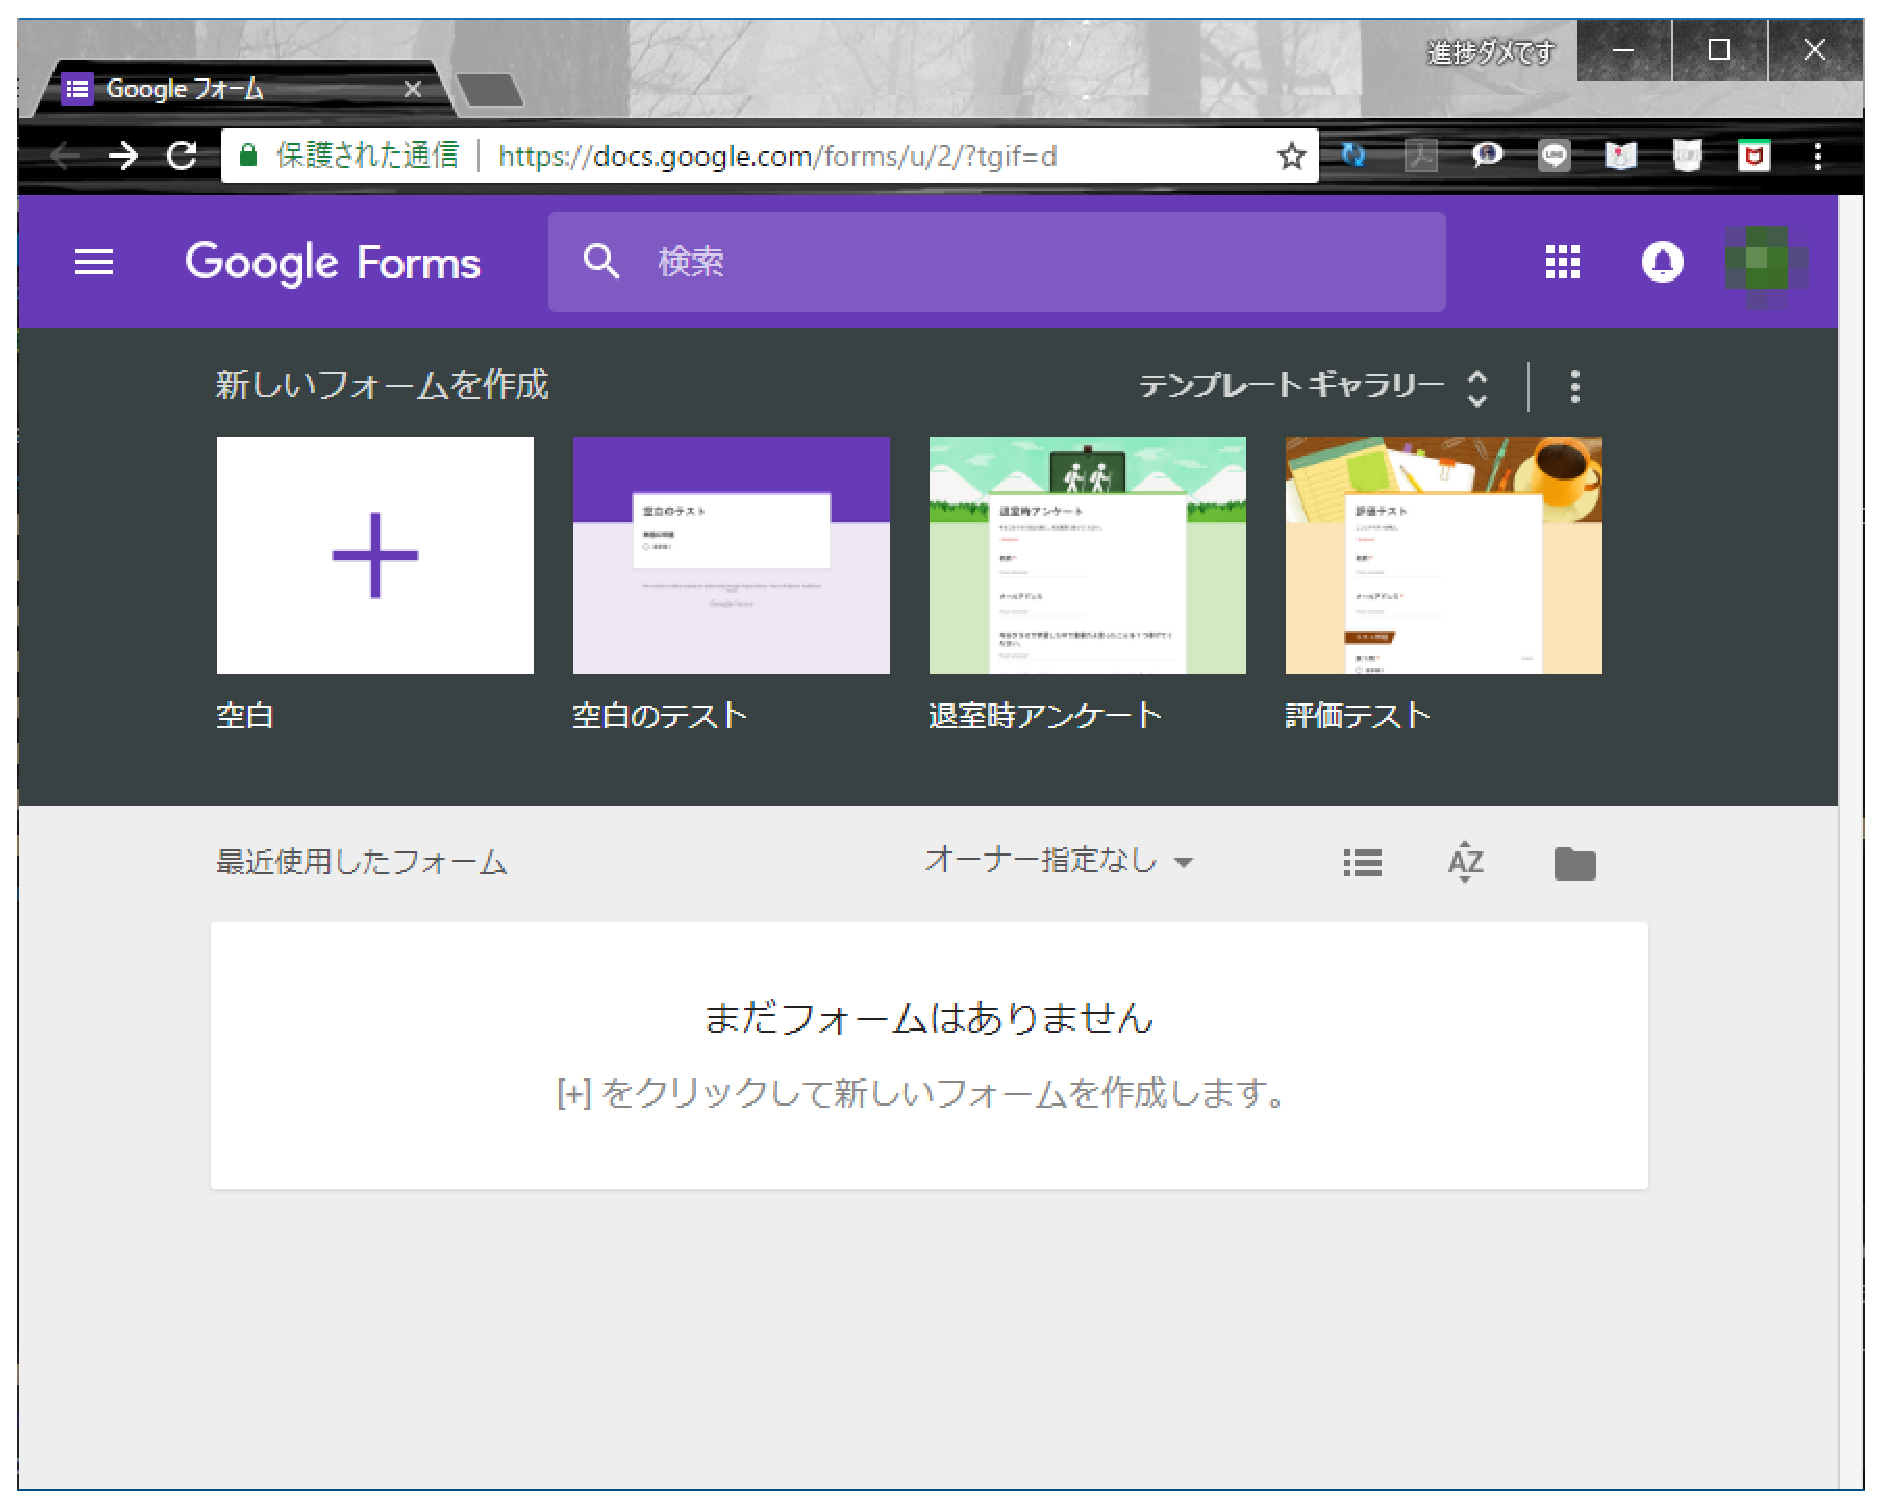
\includegraphics[width=12.0cm]{./image/form01.eps}
                            \caption{Google Forms トップページ}
                            \label{fig:form01}
                            \end{center}
                        \end{figure}

                        この時に、学内のGoogleアカウントでログインすると、フォームの回答ページにも学内アカウントのみがアクセスできるようになります。
                \item 「新しいフォームを作成」の項目からテンプレート等を選んでフォームを作成します。
                \item フォーム作成ページが出てきたら、タイトルや説明文を記述します。
                    \begin{figure}[htbp]
                        \begin{center}
                        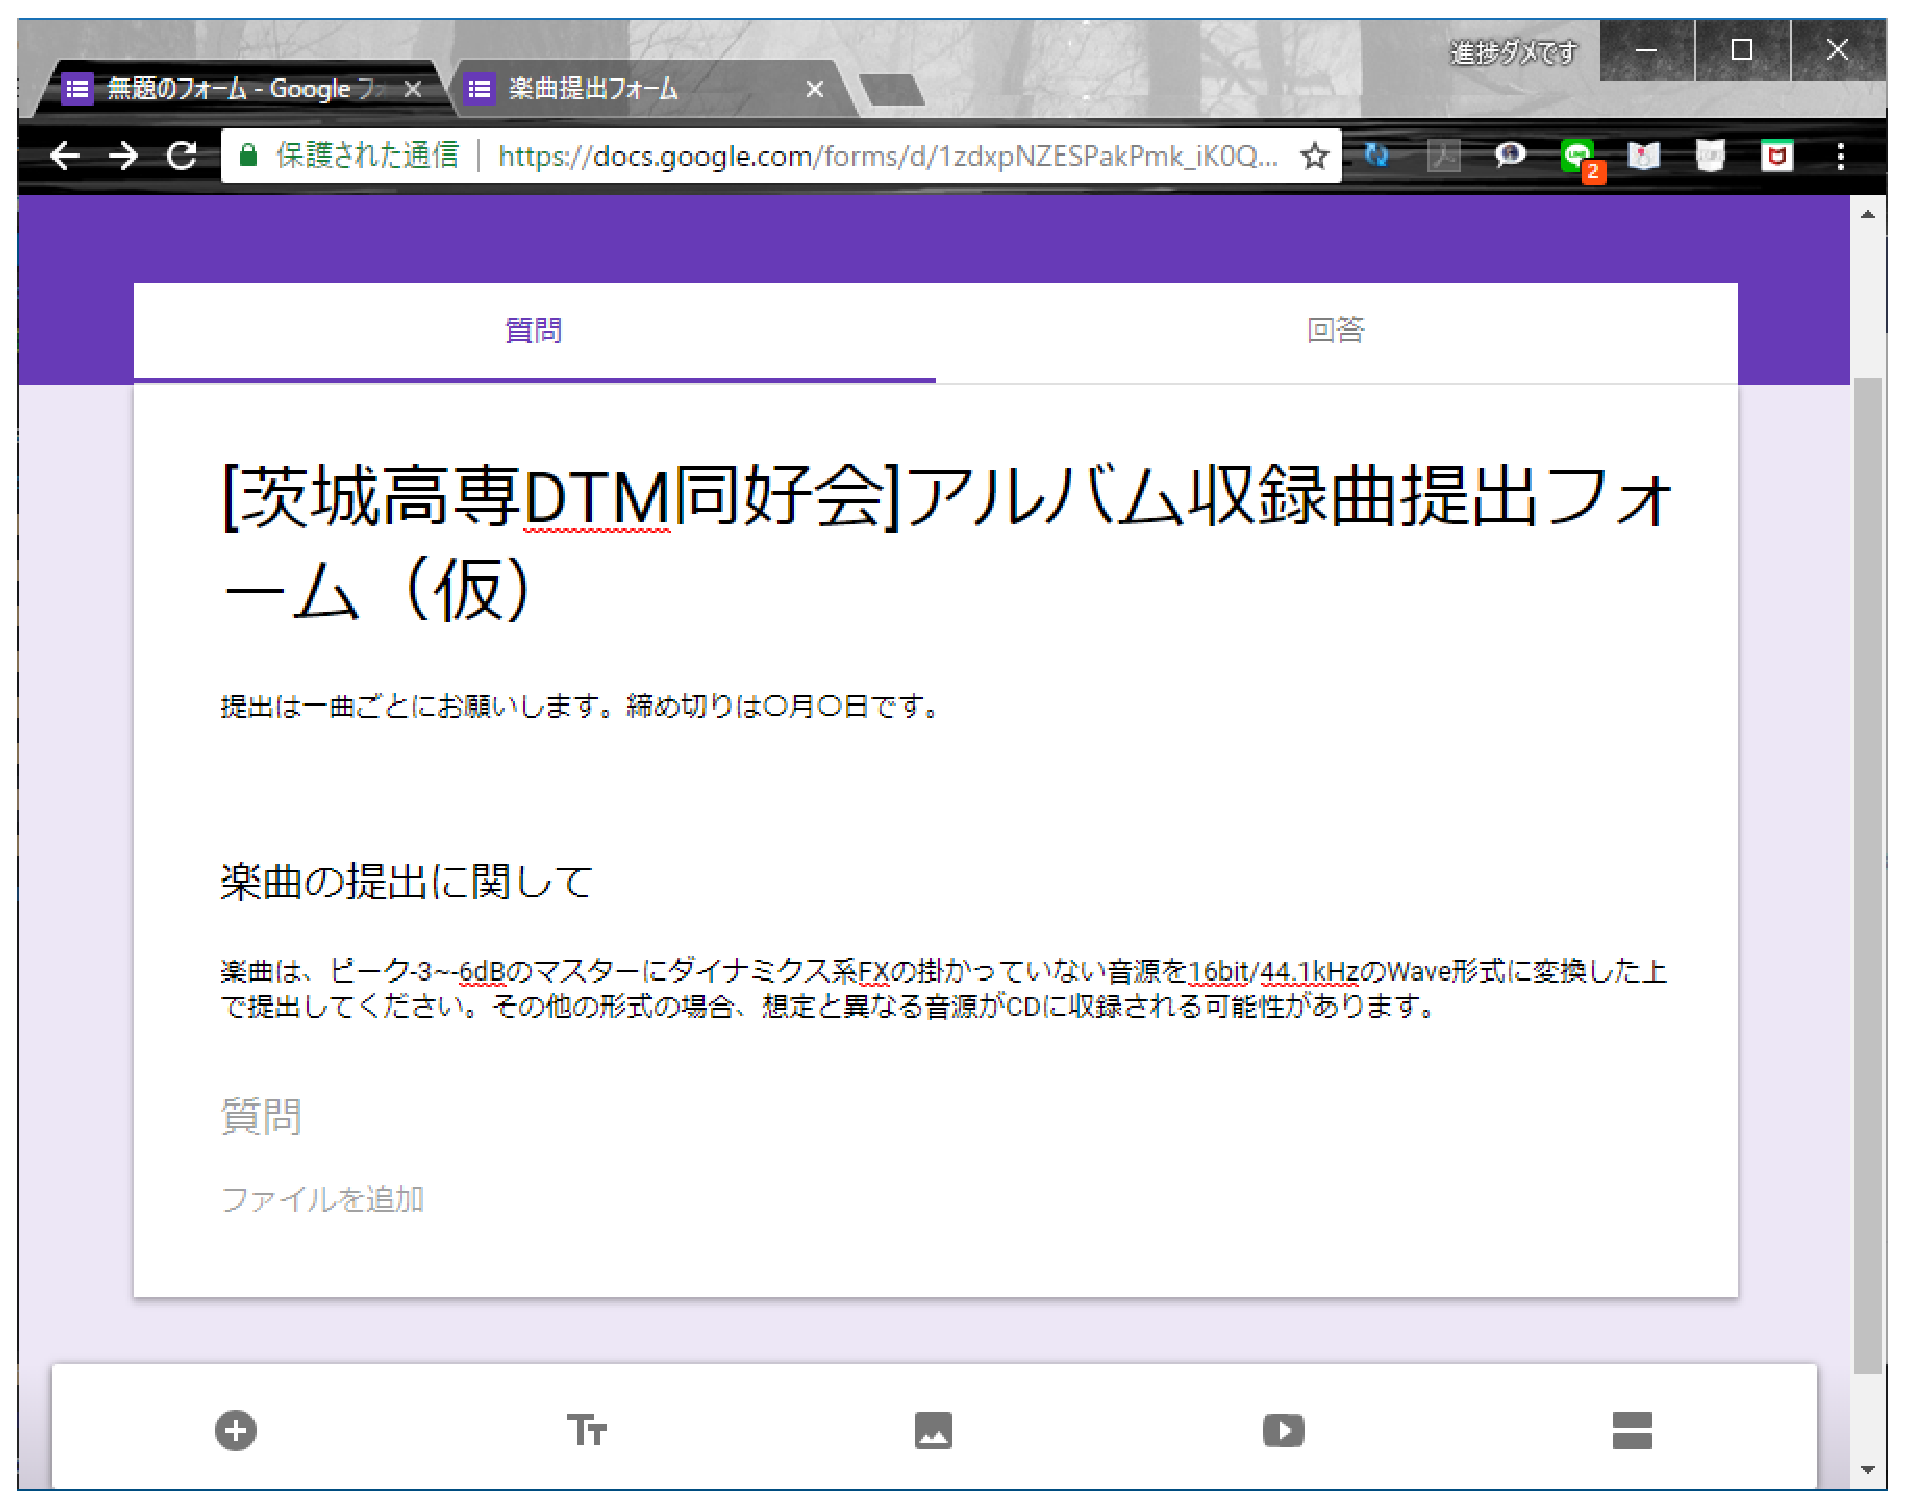
\includegraphics[width=12.0cm]{./image/form02.eps}
                        \caption{フォーム編集画面}
                        \label{fig:form02}
                        \end{center}
                    \end{figure}
                \item 下部の「質問を追加」ボタンを押して、質問項目を追加していきます。
                    \begin{figure}[htbp]
                        \begin{center}
                        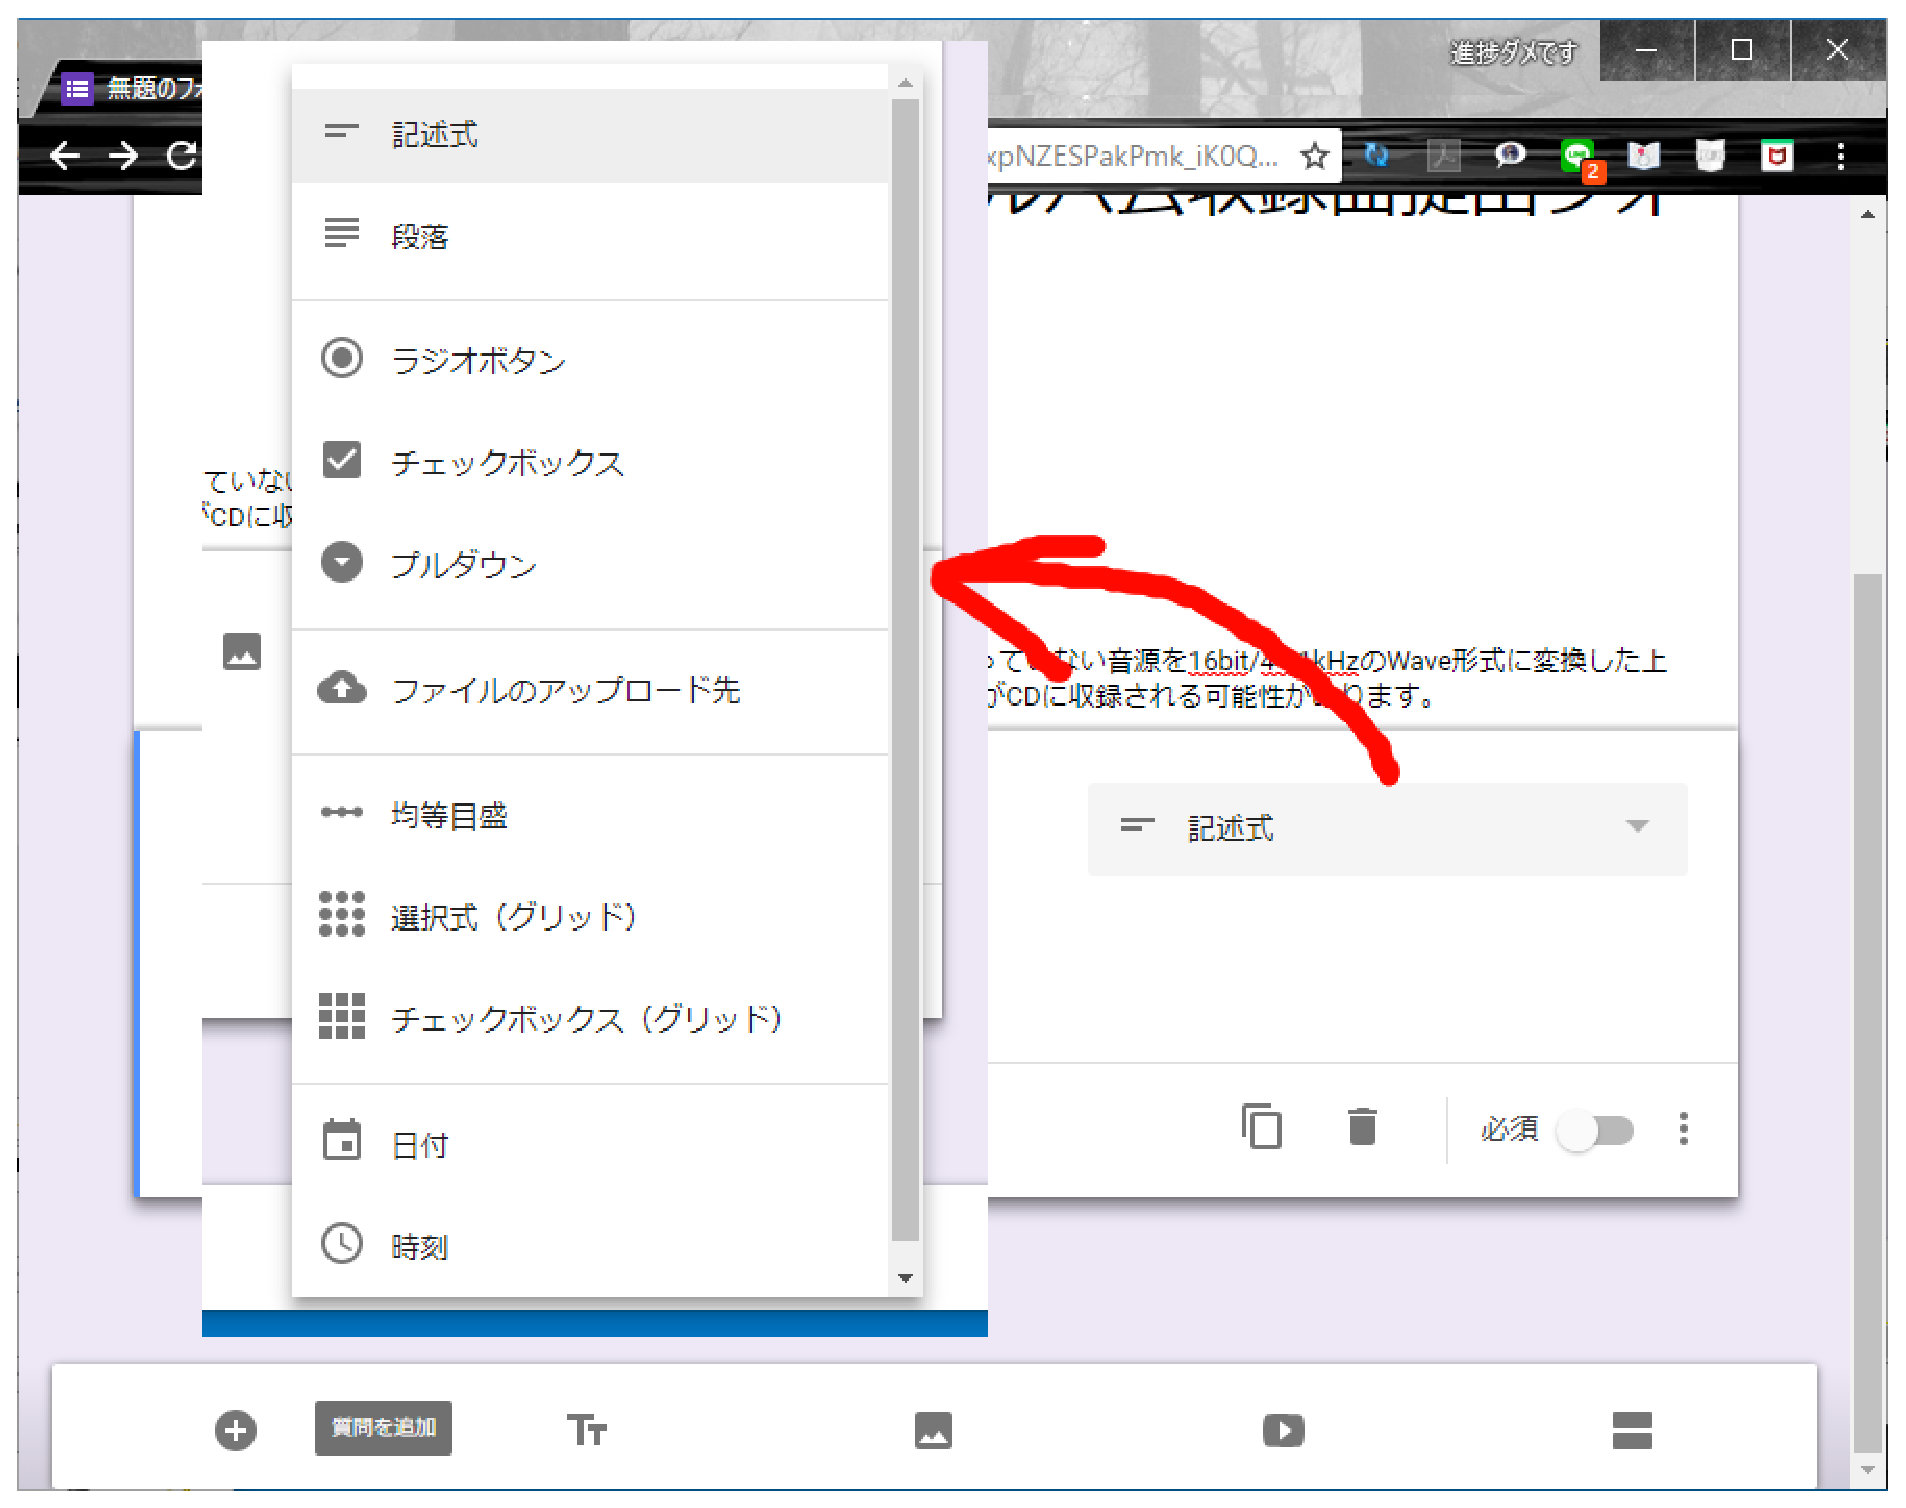
\includegraphics[width=12.0cm]{./image/form03.eps}
                        \caption{質問項目の種類}
                        \label{fig:form03}
                        \end{center}
                    \end{figure}
                    
                    質問項目の種類には様々なものがあるので、質問の内容によって使い分けます。
                    必ず回答してほしい項目は「必須」スイッチをオンにしましょう。
                    \begin{itemize}
                        \item 記述式 \\
                            一文程度の短い回答ができます。「曲のタイトル」「アーティスト名」「ジャンル」「学年・クラス・氏名」等の質問に使えます。
                        \item 段落 \\
                            改行のできる長文の回答ができます。載せられる場所があれば歌もの曲の「歌詞」等を記述してもらいましょう。
                        \item ファイルのアップロード先 \\
                            PC内のファイルをアップロードしたり、Googleドライブからファイルを選択してデータを提出することができます。
                            ファイル形式・同時アップロードファイル最大数・最大ファイルサイズに制限をかけることもできます。
                    \end{itemize}

                \item 右上の「送信」ボタンを押して、フォームのリンクを共有します。
                    「送信方法」の項目を切り替えて、メールを送信したり、リンクを取得することができます。
                    \begin{figure}[htbp]
                        \begin{center}
                        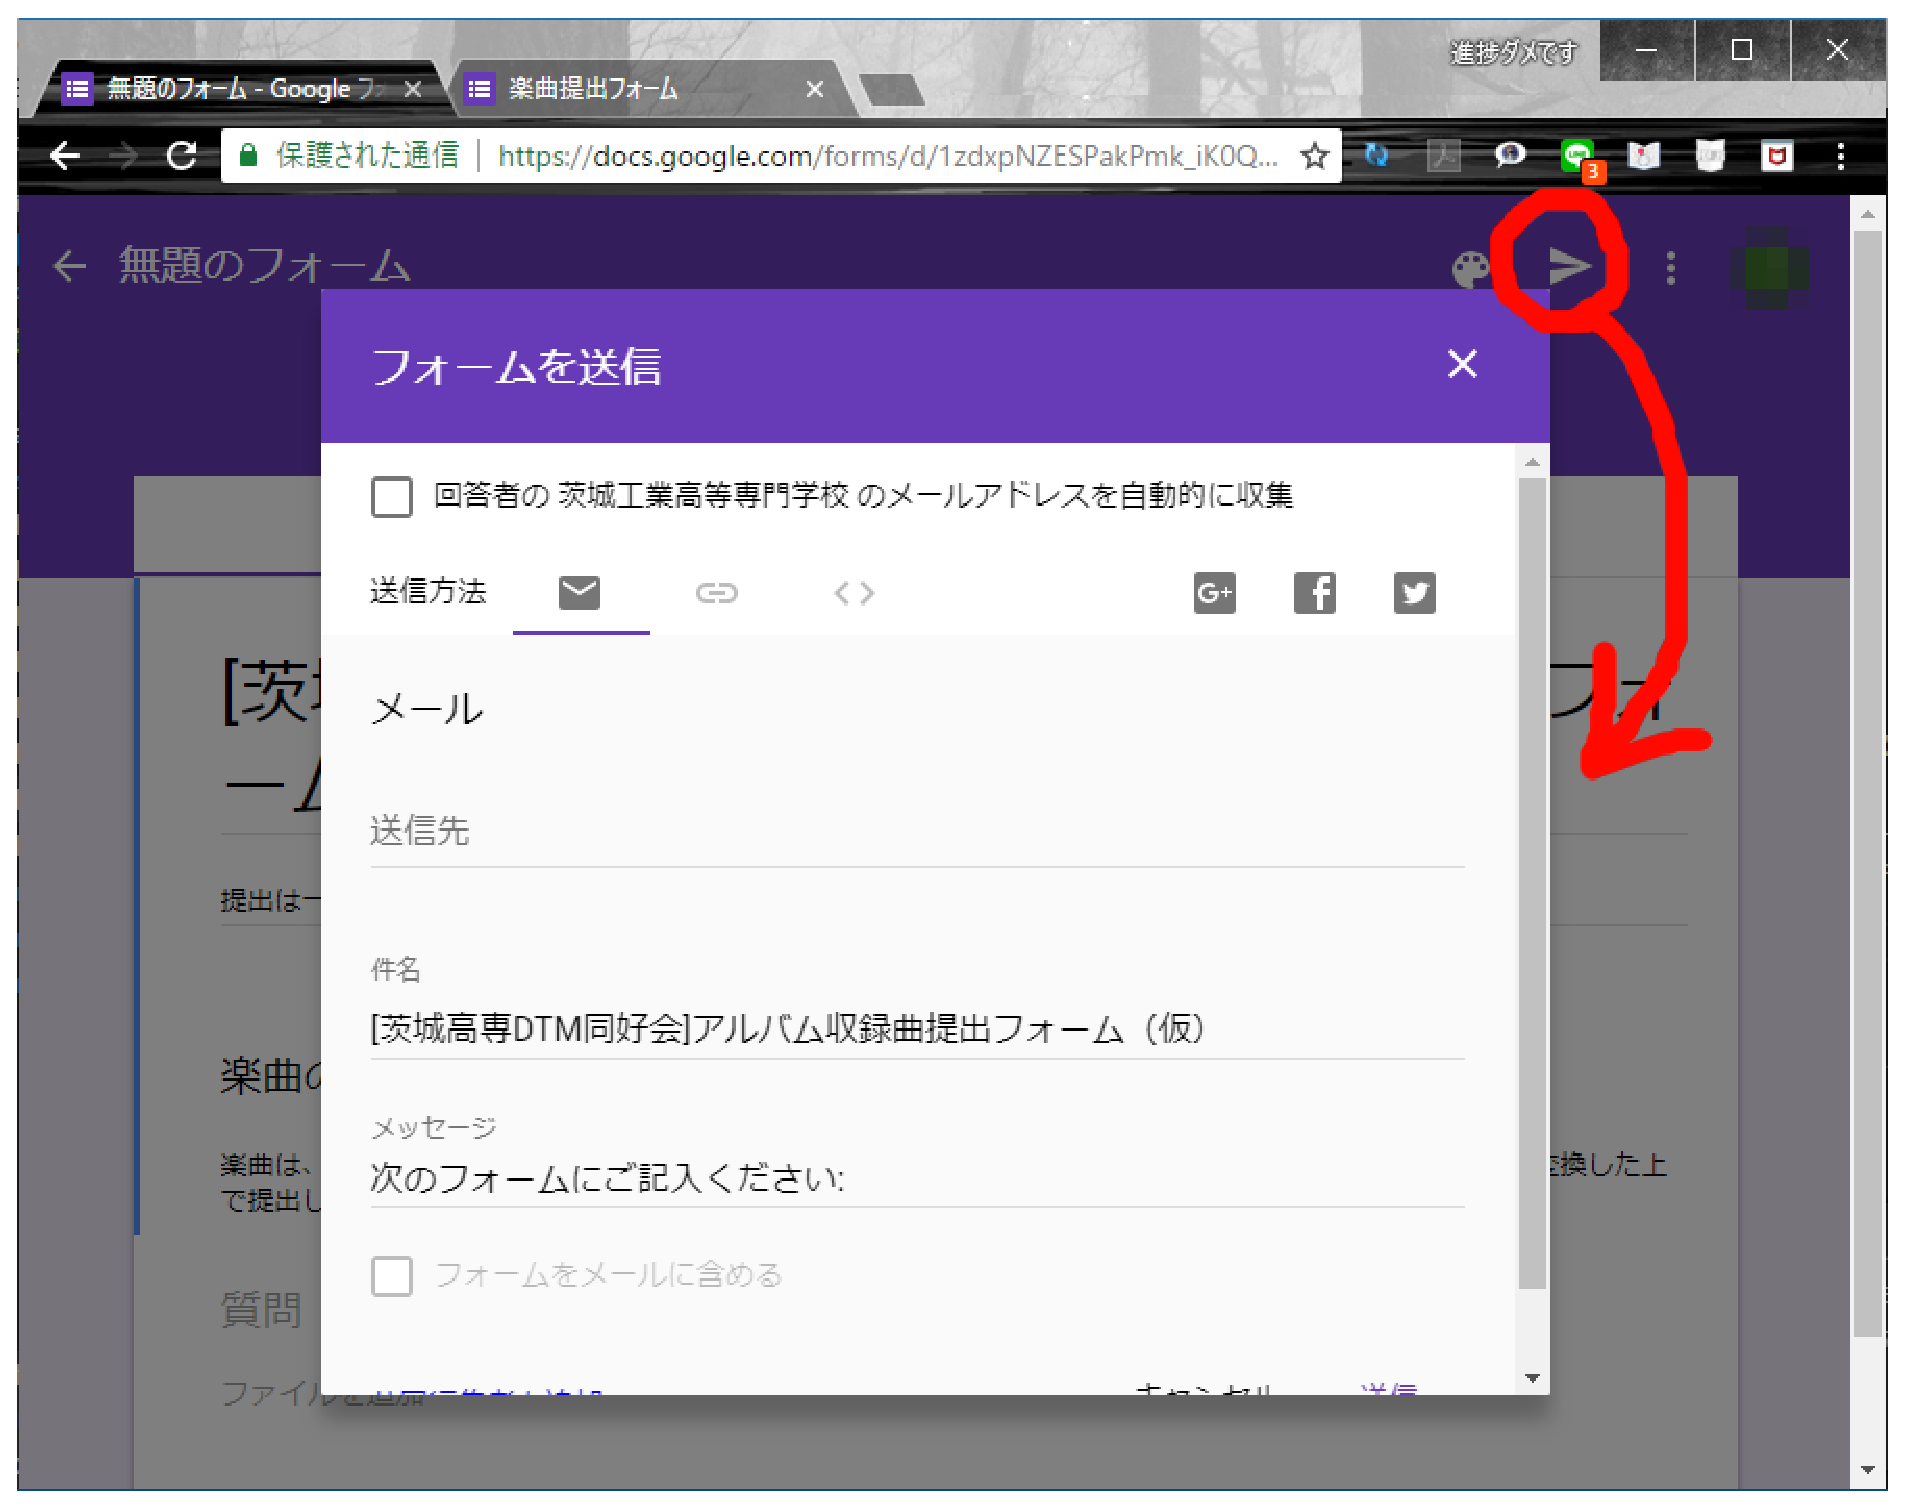
\includegraphics[width=12.0cm]{./image/form04.eps}
                        \caption{フォームの共有}
                        \label{fig:form04}
                        \end{center}
                    \end{figure}
                    メールやSNS等で部員にフォームのリンクを送信しましょう。

                \item 「回答」タブで回答を確認できます。
                    右上の「回答をスプレッドシートに表示」ボタンを押すと、表形式で回答を確認することもできます。
                    \begin{figure}[htbp]
                        \begin{minipage}{0.5\hsize}
                         \begin{center}
                          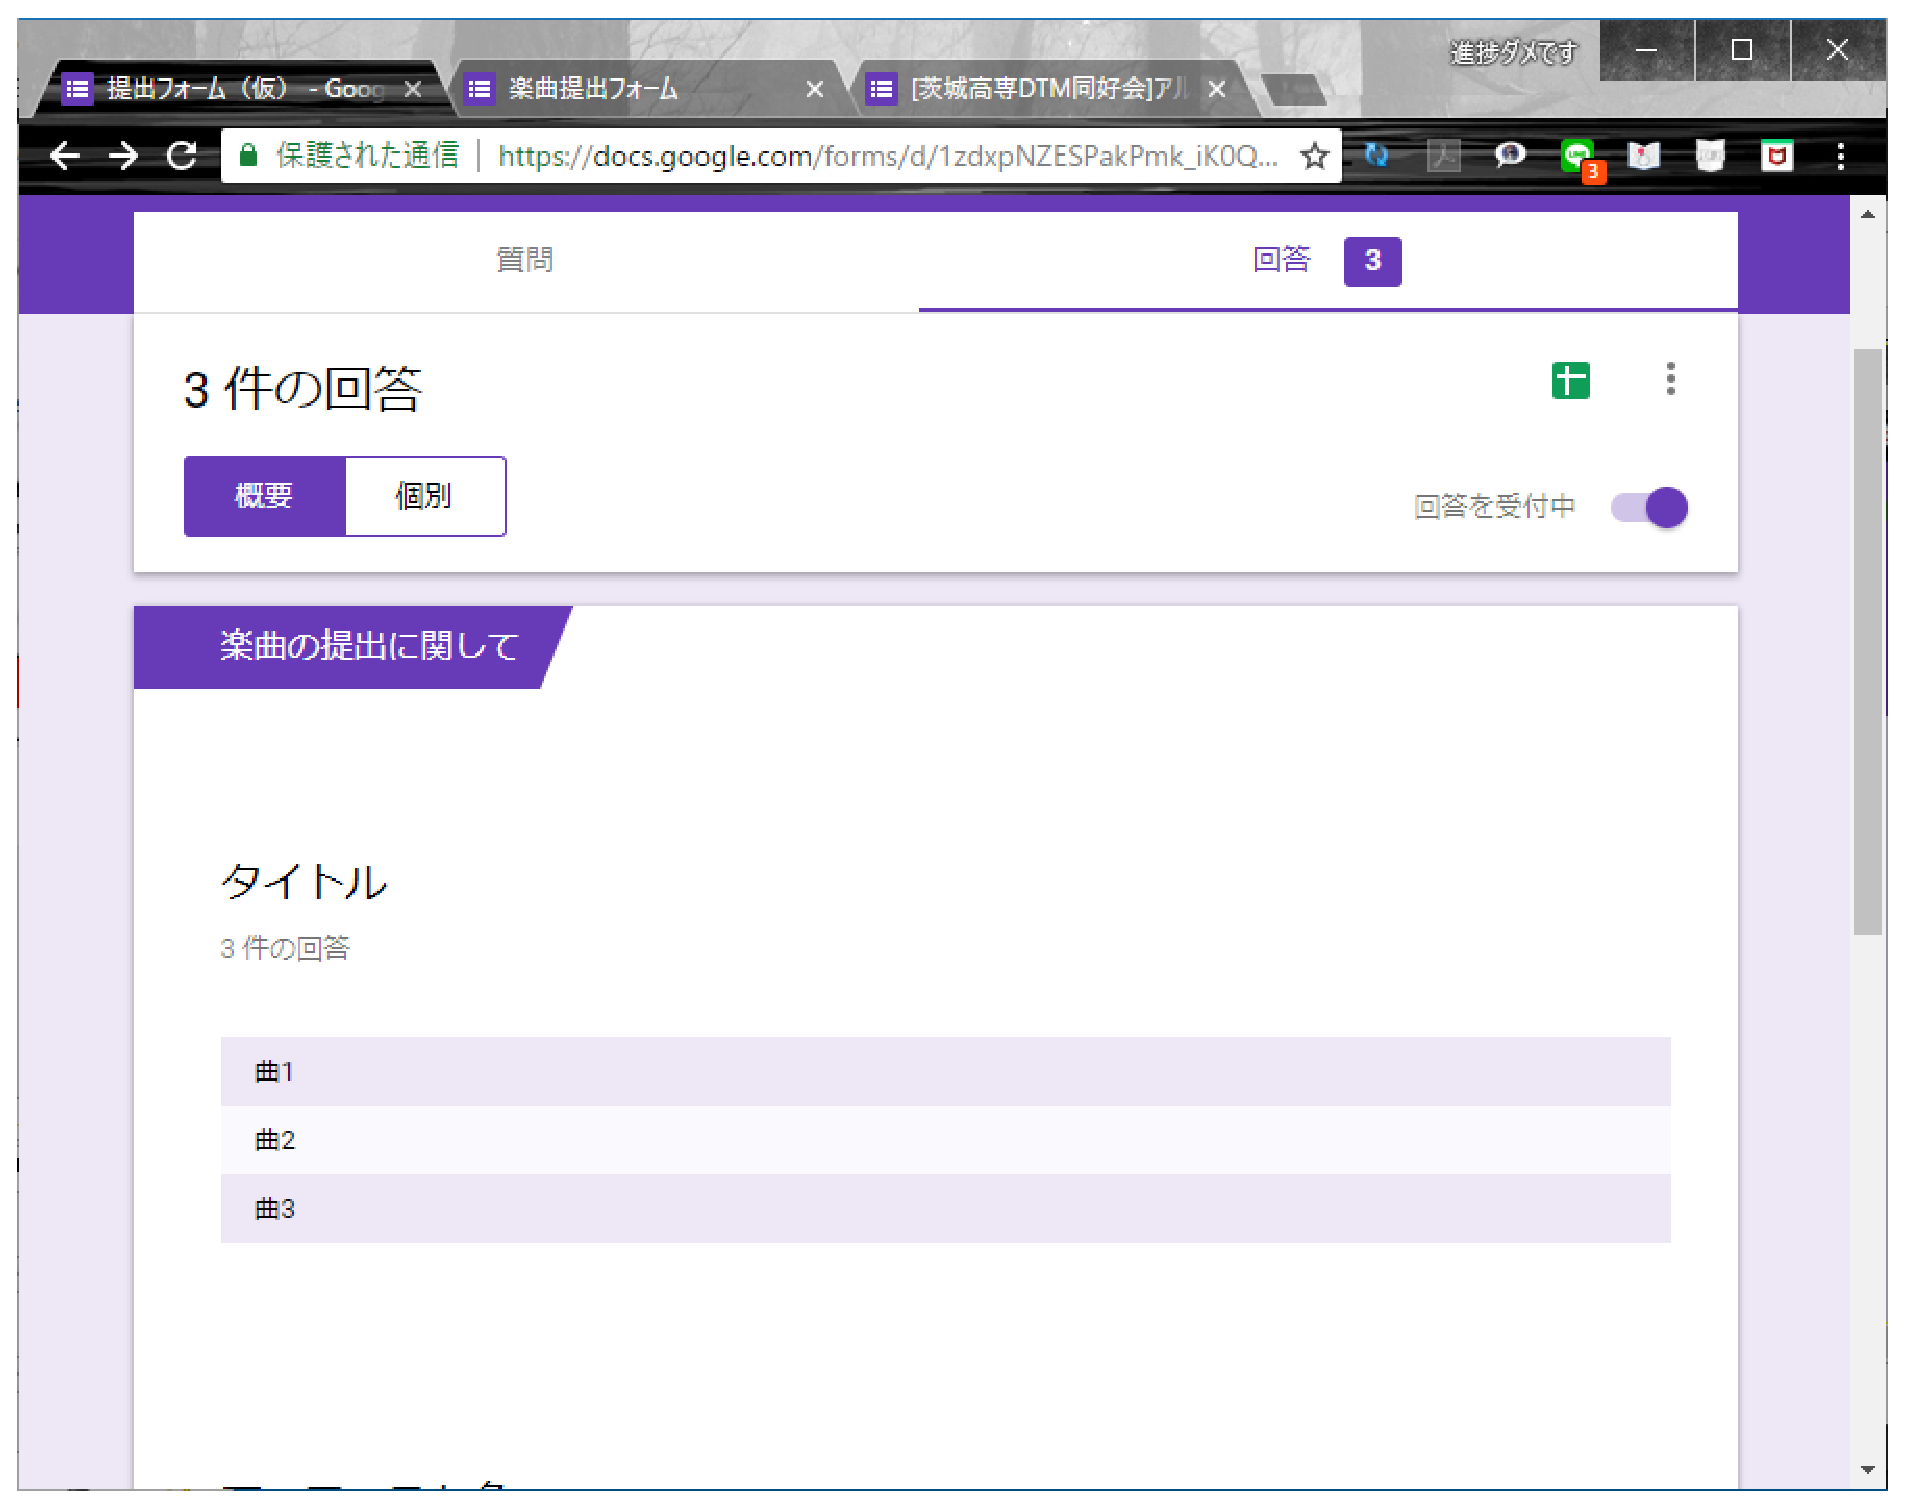
\includegraphics[width=70mm]{./image/form05.eps}
                         \end{center}
                         \caption{回答の集計}
                         \label{fig:form05}
                        \end{minipage}
                        \begin{minipage}{0.5\hsize}
                         \begin{center}
                          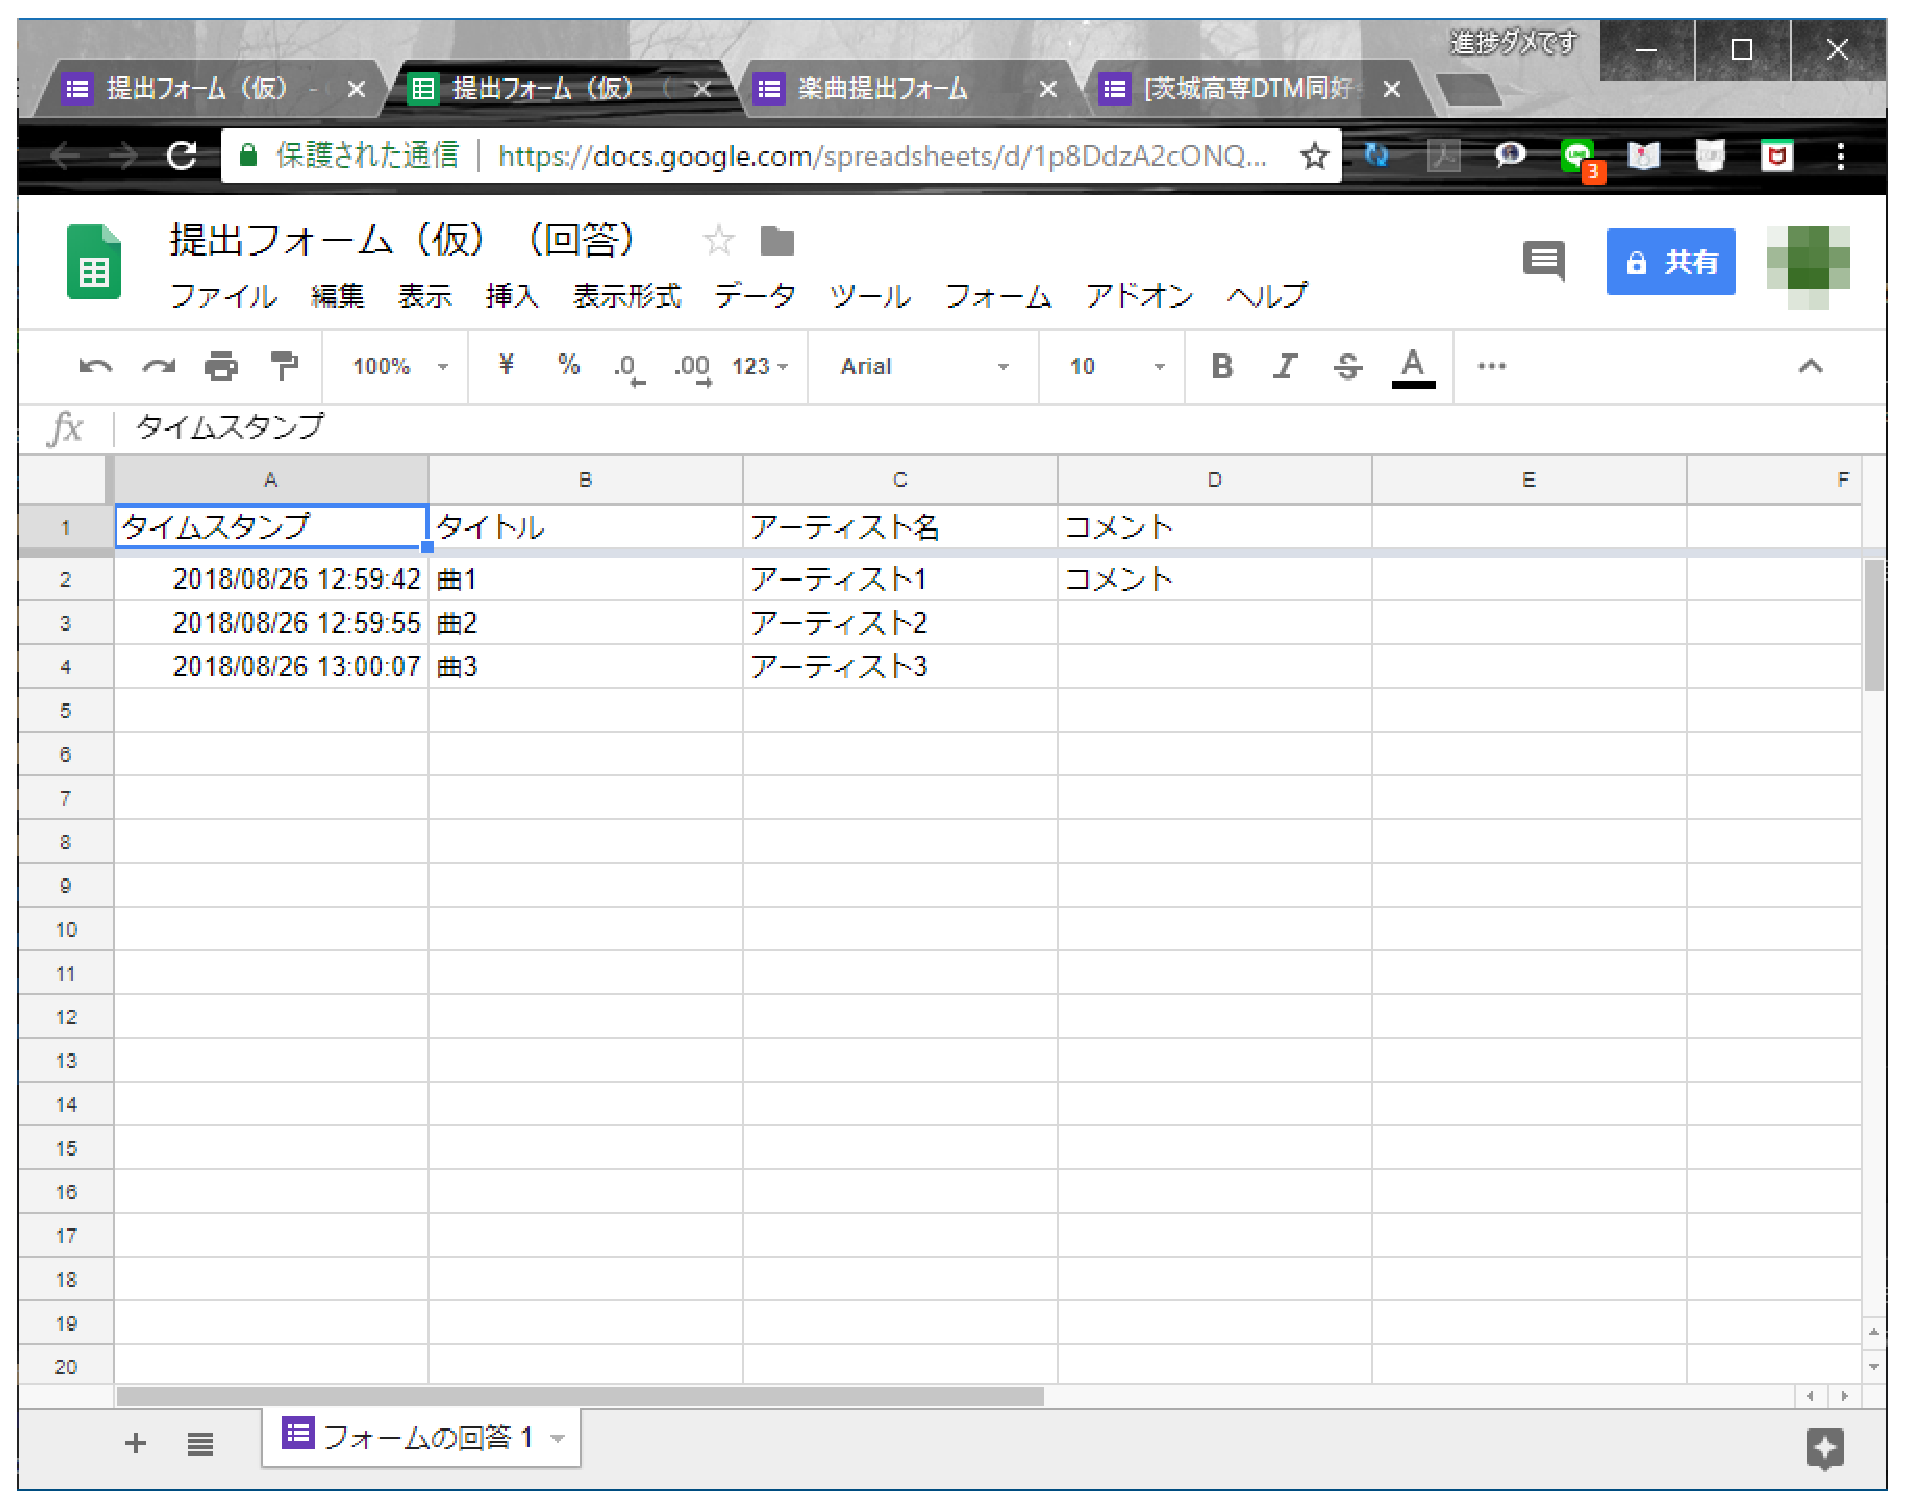
\includegraphics[width=70mm]{./image/form06.eps}
                         \end{center}
                         \caption{回答の集計(表形式)}
                         \label{fig:form06}
                        \end{minipage}
                    \end{figure}

                \end{enumerate}

            曲が集まったら、曲情報を一つのテキストファイルなどに書き出し、音声ファイルをzipにまとめてマスタリング担当者に渡しましょう。
        
        \subsection{提出形式}
            提出する曲データのファイル形式を決めておきましょう。
            マスタリング前は曲としての最良の原型が残った、よい波形で書き出すことを心がけましょう。

            \subsubsection{フォーマット:wav}
                ファイルの拡張子が「.wav」になるようにしてください。wavは最も標準的に使われている非圧縮形式の音声フォーマットで、
                マスタリングやCDに焼く際にデータの劣化が少ないです。

                Dominoなどのmidi形式(.mid)で曲を書き出すソフトを使っている人は、何かしらのDAWをインストールし
                \footnote{Studio One PrimeやFLStudio等の無料のDAWもあります。使い方は各自調べてください。}
                \begin{enumerate}
                    \item midi形式のファイルをDAWにインポートする。(大体のDAWはプロジェクトを作成した後に、その上にmidiファイルをD\&Dすれば読み込んでくれます)
                    \item トラックごとに音色を調整する
                    \item wavファイルにエクスポートする
                \end{enumerate}
                というような作業を行って、wavファイルを作成してください。

            \subsubsection{ピークレベル:-3~-6dB}
                ピークレベルとは、信号のレベルで一番高い瞬間の値を表します。
                信号が振り切れているところがあると、クリップノイズを生じてしまいます。
                マスタリングで音圧を上げられるように、提出音源はちょうどよい音量に抑えておきましょう。
                \begin{figure}[htbp]
                    \begin{center}
                    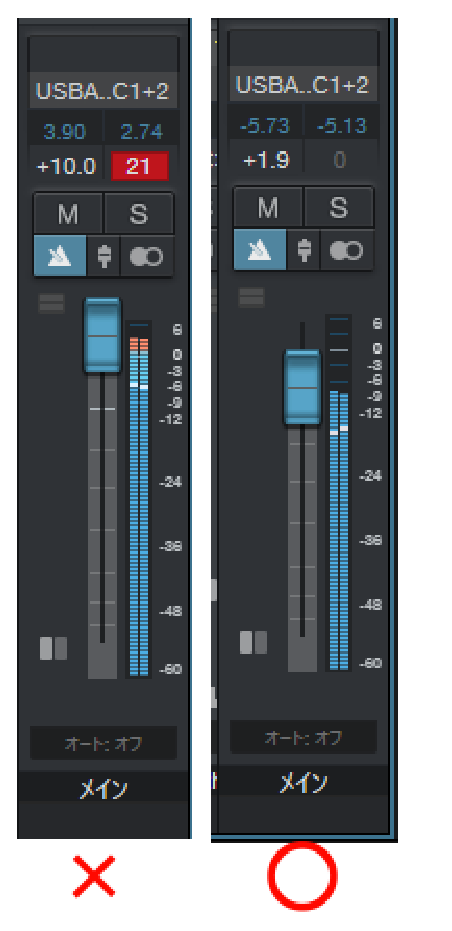
\includegraphics[width=2.0cm]{./image/format01.eps}
                    \caption{ピークレベル}
                    \label{fig:format01}
                    \end{center}
                \end{figure}

                ピークメーターはDAWのMIX画面で確認できます。
                マスタートラックのピークメーターが、赤いところまで来ていたら音量を下げてください。

            \subsubsection{マスターにはダイナミクス系FXをかけない}
                マスタートラックというのは全てのトラックの音が合わさった、曲が出力されるトラックのことを言います。
                メイン、output等DAWによって表記は異なりますが、大体MIX画面の端の方にあります。

                通常DAWはトラックごとにエフェクトがかけられるようになっていて、マスタートラックにもエフェクトをかけることができます。
                曲の音圧を上げるために、マスタートラックにマキシマイザーやコンプレッサー等のダイナミクス系エフェクトをかける人がいますが、
                曲を提出する際は、マスタリングに差し支えるので何も挿さないでください。

            \subsubsection{ビット深度:16bit}
                ビット深度は音量レベルの精度を表します。
                
                設定できる値として8bitや24bit,32bit floatがりますが、8bitは精度が低く、24bit,32bit floatは対応していないソフトなどがあるので、
                16bitにしておくのが無難です。

            \subsubsection{サンプリング周波数:44.1kHz}
                サンプリング周波数は一秒間のサンプリング回数を表します。
                \footnote{時間のグラフを考えたとき、ビット深度が縦軸、サンプリング周波数が横軸の制度にあたります。}
                
                波形を再現するには1周期最低2点の波形情報が必要で、人間が聞き取れる最低周波数が20kHzなので、
                20kHz×2=40kHzが、音を表現するのに必要最低限のサンプリング周波数となります。
                
                44.1kHzは一般的なCDのサンプリング周波数であり、ほとんどのソフトで対応しているので、これに設定しておくのが無難です。
            
            

%
%
\end{document}

%デュプリケーターの使い方